\chapter{Aplicacion}

\section{Introducción}

\newpage

\section{Aplicacion}
contenido...

\subsection{Comportamiento aplicacion}
\begin{figure}[h!]
	\centering
	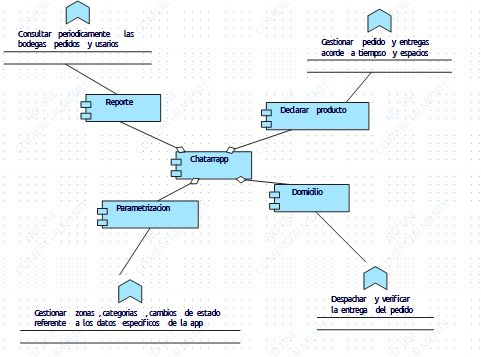
\includegraphics[width=0.8\linewidth]{Arquitectura/Aplicacion/imgs/Comportamiento aplicacion.png}
	\caption{Comportamiento}
\end{figure}
\newpage

\subsection{Cooperacion de aplicacion}
\begin{figure}[h!]
	\centering
	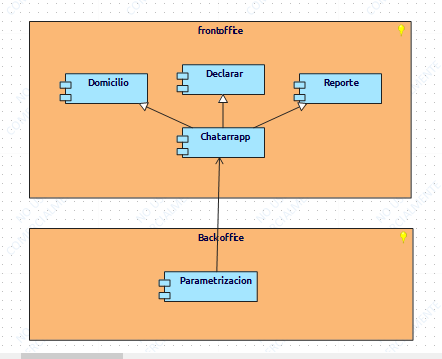
\includegraphics[width=0.8\linewidth]{Arquitectura/Aplicacion/imgs/Cooperacion de aplicacion.png}
	\caption{Cooperacion}
\end{figure}
\newpage

\subsection{Estructura de apilcacion}
\begin{figure}[h!]
	\centering
	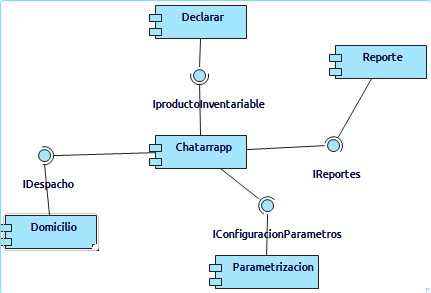
\includegraphics[width=0.8\linewidth]{Arquitectura/Aplicacion/imgs/Estructura de apilcacion.png}
	\caption{Estructura}
\end{figure}
\newpage

\subsection{uso de aplicacion}
\begin{figure}[h!]
	\centering
	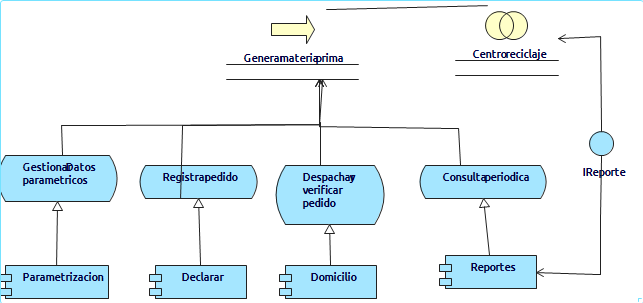
\includegraphics[width=0.8\linewidth]{Arquitectura/Aplicacion/imgs/uso de aplicacion.png}
	\caption{uso}
\end{figure}
\newpage

